%iffalse
\let\negmedspace\undefined
\let\negthickspace\undefined
\documentclass[journal,12pt,onecolumn]{IEEEtran}
\usepackage{cite}
\usepackage{amsmath,amssymb,amsfonts,amsthm}
\usepackage{algorithmic}
\usepackage{graphicx}
\usepackage{textcomp}
\usepackage{xcolor}
\usepackage{txfonts}
\usepackage{listings}
\usepackage{circuitikz}
\usepackage{enumitem}
\usepackage{mathtools}
\usepackage{pgfplots}
\usepackage{tikz}
\usepackage{gensymb}
\usepackage{comment}
\usepackage[breaklinks=true]{hyperref}
\usepackage{tkz-euclide} 
\usepackage{listings}
\usepackage{gvv}                                        
%\def\inputGnumericTable{}                                 
\usepackage[latin1]{inputenc}                                
\usepackage{color}                                            
\usepackage{array}                                            
\usepackage{longtable}                                       
\usepackage{calc}                                             
\usepackage{multirow}                                         
\usepackage{hhline}                                           
\usepackage{ifthen}                                           
\usepackage{lscape}
\usepackage{tabularx}
\usepackage{array}
\usepackage{float}

\usepackage{enumitem}
\usepackage{xcolor}
%\usepackage{multicol}


\newtheorem{theorem}{Theorem}[section]
\newtheorem{problem}{Problem}
\newtheorem{proposition}{Proposition}[section]
\newtheorem{lemma}{Lemma}[section]
\newtheorem{corollary}[theorem]{Corollary}
\newtheorem{example}{Example}[section]
\newtheorem{definition}[problem]{Definition}
\newcommand{\BEQA}{\begin{eqnarray}}
\newcommand{\EEQA}{\end{eqnarray}}
\newcommand{\define}{\stackrel{\triangle}{=}}
\theoremstyle{remark}
\newtheorem{rem}{Remark}

\title{2017-XE-27-39}
\author{AI24BTECH11023 - Tarun Reddy Pakala}
\begin{document}
\bibliographystyle{IEEEtran}

\maketitle
\bigskip
\renewcommand{\thefigure}{\theenumi}
\renewcommand{\thetable}{\theenumi}
\begin{enumerate}[start=27]
\item The stream function $\brak{\Psi}$ of a velocity field at any location \brak{x,\;y} is given as, $\Psi=xy^2-2x^2y^2$. What is the rate of rotation of a fluid element located at \brak{x=2,y=2}?
\begin{enumerate}
    \item $8$
    \item $10$
    \item $12$
    \item $14$
\end{enumerate}
\item The nature of velocity profile within the laminar viscous sublayer in a turbulent pipe flow is
\begin{enumerate}
    \item linear 
    \item parabolic
    \item logarithmic
    \item exponential
\end{enumerate}
\item In a $5\;m$ deep vertical cylindrical tank, water is filled up to a level of $3\;m$ from the bottom and the remaining space is filled with oil of specific gravity $0.88$. Assume density of water as $1000\;\frac{kg}{m^3}$ and acceleration due to gravity to be $10\;\frac{m}{s^2}$. The gauge pressure \brak{\text{in} \;\frac{kN}{m^2}, \text{rounded off to the first decimal place}} at a depth of $2.5\;m$ from the top of the tank will be \underline{\hspace{2cm}}.
\item In a two-dimensional potential flow, a point source is located at the origin \brak{x=0,\;y=0} as shown in the figure. The strength of the point source is $2\;\frac{cm^2}{s}$. A uniform flow with velocity $1\frac{cm}{s}$ is approaching towards the point source at an angle of $30\degree$ from the horizontal axis. What is the distance \brak{cm} of the stagnation point in the flow field from the point source?
%input for figure 1
	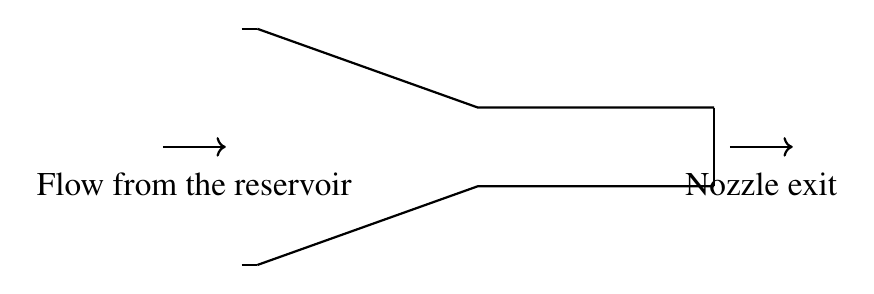
\begin{tikzpicture}
    % Draw the nozzle shape with short vertical lines at the opening
    \draw[thick] (-3,1.5) -- (-2.8,1.5);
    \draw[thick] (-3,-1.5) -- (-2.8,-1.5);
    \draw[thick] (-2.8,1.5) -- (0,0.5) -- (3,0.5);
    \draw[thick] (-2.8,-1.5) -- (0,-0.5) -- (3,-0.5);
    
    % Vertical line at the nozzle exit
    \draw[thick] (3,0.5) -- (3,-0.5);

    % Flow direction arrows
    \draw[->, thick] (-4,0) -- (-3.2,0);
    \draw[->, thick] (3.2,0) -- (4,0);

    % Labels for the flow and nozzle exit, placed below arrows
    \node[below] at (-3.6,-0.2) {\large Flow from the reservoir};
    \node[below] at (3.6,-0.2) {\large Nozzle exit};
\end{tikzpicture}

	\begin{enumerate}
    \item $\frac{1}{\pi}$
    \item $\frac{2}{\pi}$
    \item $\frac{1}{2\pi}$
    \item $\frac{\sqrt{3}}{2\pi}$
\end{enumerate}
\item Two infinite parallel horizontal plates are separated by a small gap \brak{d=20\;mm} as shown in figure. The bottom plate is fixed and the gap between the plates is filled with oil having density of $890\;\frac{kg}{m^3}$ and kinematic viscosity of $0.00033\frac{m^2}{s}$. A shear flow is induced by moving the upper plate with a velocity of $5 \frac{m}{s}$. Assume, linear velocity profile between and the plates and the oil to be a Newtonian fluid. The shear stress \brak{\frac{N}{m^2}} at the upper plate is \underline{\hspace{2cm}}
%input for figure 2
	\begin{figure}[!ht]
\centering
\resizebox{3cm}{3cm}{%
\begin{circuitikz}
\tikzstyle{every node}=[font=\LARGE]
\draw [ line width=0.6pt](2.75,12) to[sinusoidal voltage source, sources/symbol/rotate=auto] (3.25,11.5);
\draw [ line width=0.6pt](3.25,11.75) to[european resistor] (9.5,11.75);
\draw [line width=0.6pt, ->, >=Stealth] (9.5,11.75) -- (9.5,11);
\draw [ line width=0.6pt](4,12.25) to[short] (4,11.25);
\draw [ line width=0.6pt](4,11.5) to[short] (4,11);
\draw [ line width=0.6pt](8.75,12.25) to[short] (8.75,11);
\draw [ line width=0.6pt](4,11.25) to[short] (4.5,11.25);
\draw [ line width=0.6pt](8.75,11.25) to[short] (8.25,11.25);
\draw [ line width=0.6pt](4.25,11.25) to[short] (5.25,11.25);
\draw [ line width=0.6pt](8.25,11.25) to[short] (7.25,11.25);
\draw [ line width=0.6pt](5,11.25) to[european resistor] (5,8.5);
\draw [ line width=0.6pt](7.5,11.25) to[european resistor] (7.5,8.5);
\draw [ line width=0.6pt](4.75,8.5) to[short] (8,8.5);
\draw [line width=0.6pt, ->, >=Stealth] (6.25,8.5) -- (6.25,7.75);
\node [font=\normalsize] at (6.75,8) {Bus 3};
\node [font=\normalsize] at (4,12.5) {Bus 1};
\node [font=\normalsize] at (8.75,12.5) {Bus 2};
\node [font=\normalsize] at (6.25,12.25) {j q};
\node [font=\normalsize] at (4.5,10) {j r};
\node [font=\normalsize] at (8.25,9.75) {j p};
\end{circuitikz}
}%

\label{fig:my_label}
\end{figure}

\item A spherical balloon of diameter $15\;m$ is supposed to lift a load of $3000\;N$. The lifting of load is achieved by heating the air inside the balloon. Assume, air to be an ideal gas and the atmospheric pressure either outside or inside the balloon. The value of acceleration due to gravity is $9.81\;\frac{m}{s^2}$ and the values of temperature and density of atmospheric air are $15\degree C$ and $1.2\;\frac{kg}{m^3}$, respectively. In order to lift the specified load, the air inside the balloon should be heated to a temperature \brak{\degree C} of \underline{\hspace{2cm}} 
\item The velocity field in Cartesian coordinate system for a two-dimensional steady flow is given as : $$\overrightarrow{V}=\brak{\frac{V_o}{L}}\brak{x \hat{i}-y \hat{j}}$$ where, $V_o$ and $L$ are constants. Which one of the following expressions represents the acceleration field \brak{\overrightarrow{a}} for this flow?
\begin{enumerate}
    \item $\dot{a}=0$
    \item $\overrightarrow{a}=\brak{\frac{V_o}{L}}\brak{x\;\hat{i}+y\;\hat{j}}$
    \item $\dot{a}=\brak{\frac{V_o^2}{L^2}}\brak{x\;\hat{i}-y\;\hat{j}}$
    \item $\dot{a}=\brak{\frac{V_o^2}{L^2}}\brak{x\;\hat{i}+y\;\hat{j}}$
\end{enumerate}
\item A cylindrical tank of $0.8\;m$ diameter is completely filled with water and its top surface is open to atmosphere as shown in the figure. Water is being discharged to the atmosphere from a circular hole of $15\;mm$ diameter located at the bottom of the tank. The value of acceleration due to gravity is $9.81\;\frac{m}{s^2}$. How much time \brak{\text{in seconds}} would be required for the water level to drop from a height of $1\;m$ to $0.5\;m$ ?  
%input for figure 3
\begin{figure}[!ht]
\centering
\resizebox{3cm}{3cm}{%
\begin{circuitikz}
\tikzstyle{every node}=[font=\small]
\draw (4.25,12.25) to[battery1] (4.25,7.75);
\draw (4.25,12.25) to[short] (6.25,12.25);
\draw (4.25,7.75) to[short] (6.25,7.75);
\draw (6.25,12.25) to[R] (6.25,10.25);
\draw (6.25,10.25) to[R] (6.25,7.75);
\draw (6.25,10.25) to[short] (8.75,10.25);
\draw (6.25,7.75) to[short] (8.75,7.75);
\draw (8.75,7.75) to[R] (8.75,9.25);
\draw (8.75,10.25) to[D] (8.75,9);
\node [font=\small] at (4,10.25) {+};
\node [font=\small] at (4,9.75) {-};
\node [font=\small] at (4.75,10.5) {24 Volt};
\node [font=\small] at (6.75,11.25) {12 k$\Omega$};
\node [font=\small] at (6.75,9) {6 k$\Omega$};
\node [font=\small] at (8,8.5) {3.3 k$\Omega$};
\end{circuitikz}
}%

\label{fig:my_label}
\end{figure}

	\begin{enumerate}
    \item $188$
    \item $266$
    \item $376$
    \item $642$
\end{enumerate}
\item Consider steady laminar flow of an incompressible Newtonian fluid between two infinite parallel plates, separated by a distance of $1\;m$, as shown in the figure. The bottom plate is stationary but the top one is moving in positive $x$-direction with a velocity of $3\frac{m}{s}$. The fluid pressure gradient in the flow direction is : $\frac{\partial P}{\partial x}=-18\;\frac{N}{m^3}$. If the viscosity of the fluid is $1\;kgm^{-1}s^{-1}$ then the distance of the point of maximum velocity \brak{\text{in meters, rounded off to the second decimal place}} from the bottom plate would be \underline{\hspace{2cm}}
%input for figure 4
	\begin{figure}[H]
\centering
\resizebox{3cm}{3cm}{%
\begin{circuitikz}
\tikzstyle{every node}=[font=\small]
\draw [->, >=Stealth] (3.5,10.75) -- (3.5,13.75);
\draw [->, >=Stealth] (3.5,10.75) -- (10.75,10.75);
\draw [->, >=Stealth] (2.25,10.75) -- (3.25,10.75);
\draw [dashed] (4.5,13.25) -- (4.5,8.25);
\draw [dashed] (7.25,13.25) -- (7.25,8.25);
\draw [dashed] (10,13.25) -- (10,8.25);
\draw [dashed] (2,8.25) -- (10,8.25);
\draw [dashed] (2,13) -- (10,13);
\draw [short] (4.5,10.75) -- (7.25,11.75);
\draw [short] (7.25,11.75) -- (10,9.75);
\draw [short] (4.5,10.75) -- (10,9.75);
\node [font=\small] at (2.5,11) {$M>1$};
\node [font=\small] at (3.5,14) {$y$};
\node [font=\small] at (11,10.75) {$x$};
\node [font=\small] at (4.5,8) {$X_A$};
\node [font=\small] at (7.25,8) {$X_B$};
\node [font=\small] at (10,8) {$X_C$};
\node [font=\small] at (1.75,8.25) {$Y_{II}$};
\node [font=\small] at (1.75,13) {$Y_I$};
\node [font=\small] at (5.5,11) {$\alpha$};
\node [font=\small] at (6.5,10.5) {$\alpha$};
\node [font=\small] at (9,10) {$2\alpha$};
\end{circuitikz}
}%
\label{fig:my_label}
\end{figure}

\item An inviscid incompressible fluid of density $1000\;\frac{kg}{m^3}$ is flowing in a horizontal pipe of tapered cross-section with a flow rate of $4000\;\frac{cm^3}{s}$. The area of cross-section at two different location 'A' and 'B' are $10\;cm^2 \;\text{and} \;20\;cm^2$, respectively. The velocity of the fluid at the location 'A' is $4\frac{m}{s}$ and the pressure is $5\frac{N}{m^2}$. The pressure $\brak{\frac{N}{m^2}}$ at the location 'B' would be \underline{\hspace{2cm}}
\item A viscous, incompressible and Newtonian fluid flowing through the main branch of a circular pipe bifurcates into two daughter branches whose radii are $4\;cm$ and $2\;cm$, respectively. The flow in both the daughter branches are laminar and fully developed. If the pressure gradients in both the daughter branches are same, then fraction of total volumetric flow rate \brak{\text{rounded off to the second decimal place}} coming out from the branch with $4\;cm$ diameter is \underline{\hspace{2cm}} 
%input for figure 5
	\begin{figure}[!ht]
\centering
\resizebox{3cm}{3cm}{%
\begin{circuitikz}
\tikzstyle{every node}=[font=\small]
\draw [line width=0.6pt, short] (4,10.75) -- (8.25,10.75);
\draw [line width=0.6pt, short] (8.25,10.75) -- (9.75,12);
\draw [line width=0.6pt, short] (8.25,10.25) -- (9.75,11.5);
\draw [line width=0.6pt, short] (8.25,10.25) -- (9.75,9.25);
\draw [line width=0.6pt, short] (4,9.75) -- (8.25,9.75);
\draw [line width=0.6pt, ->, >=Stealth] (9.75,11.75) -- (10.25,12.25);
\draw [line width=0.6pt, ->, >=Stealth] (9.5,9) -- (10,8.5);
\draw [line width=0.6pt, ->, >=Stealth] (3.75,10.25) -- (5,10.25);
\node [font=\small] at (3.5,10.25) {$Q$};
\node [font=\small] at (10.5,12.5) {$Q_1$};
\node [font=\small] at (10.25,8.25) {$Q_2$};
\draw [line width=0.6pt, short] (8.25,9.75) -- (9.25,9);
\end{circuitikz}
}%

\end{figure}

\item The volumetric flow rate \brak{Q} of a triangular notch is a function of the upstream liquid surface elevation \brak{H} measured form the bottom of the notch, acceleration due to gravity \brak{g}, notch angle \brak{\phi} and the approach velocity \brak{V}. Which one of the following is the correct expression for $Q$ ?
\begin{enumerate}
    \item $Q=H^\frac{1}{2}f\brak{\frac{V}{\sqrt{H}},\phi\sqrt{g}}$
    \item $Q=H f\brak{\frac{V}{\sqrt{H}},\phi\sqrt{g}}$
    \item $Q=H^\frac{3}{2}f\brak{\frac{V}{\sqrt{H}},\phi\sqrt{g}}$
    \item $Q=H^\frac{5}{2}f\brak{\frac{V}{\sqrt{H}},\phi\sqrt{g}}$
\end{enumerate}
\item Model tests are to be carried out to study the flow through a large prototype value of $0.6\;m$ diameter at a flow rate of $10\;\frac{m^3}{s}$. The same working fluid is used for both the model and the prototype. A complete geometric similarity is maintained between the model and the prototype. If the valve diameter of the model is $80\;mm$, its required flow rate $\brak{\text{in}\;\frac{m^3}{s},\;\text{rounded off to the first decimal place}}$ would be \underline{\hspace{2cm}} 
\end{enumerate}
\end{document}
